\section{Introduction}\label{s:intro}

% scheduling is good
Internet content providers often want to specify scheduling policies for their traffic. 
For example, a video streaming company might benefit from weighted fair queueing across its video traffic to its many different users sharing a bottleneck. Alternately, a web site might want to prioritize interactive web traffic (e.g., e-commerce) over bulk file transfers. 
There exists a vast literature on mechanisms for such scheduling and queue management policies~\cite{diffserv, fair-queueing, sfq, pie, CoDel, fifoplus, virtualClocks, csfq, drr, red, ecn}.
These mechanisms can decrease average flow-completion times, ensure low packet delays, isolate classes of traffic from each other, and more.

% can't scehdule today
The most effective place to enforce a scheduling policy is where queue buildup occurs; where there is queueing, there is the opportunity to reorder packets. Such links with queue build-up are often outside the control of individual content 
providers~\cite{inferring-interdomain-congestion, isp-throttle-1, isp-throttle-2, isp-throttle-3}, which prevents them from enjoying the benefits of scheduling.
%content providers and end users have been unable to enjoy the benefits of scheduling policies. 

% ISP's cant solve problem (e.g. with CSFQ)
ISPs, on the other hand, do control the bottleneck links in their carrier networks where different scheduling and queue management policies can be effectively enforced. 
However, ISPs neither have enough visibility into their customers' traffic to choose desired policies on their queues, nor enough incentives to enforce them\footnote{The case for private WANs is different, since they are owned by a single entity, and have, thus, been successful in exploiting the benefits of scheduling~\cite{swan, b4, bwe}. Our focus is public networks.}. Even if an ISP isolates each its customers' traffic (\eg with fair queueing~\cite{fair-queueing}), that still does not serve a customer's desire to enforce different scheduling policies within its own traffic.  
Large customers might be able to negotiate expensive deals with certain carriers to enforce specific policies~\cite{att-qos}. 
However, it might not be possible to negotiate such deals with \emph{all} carriers in the traffic's path, and content providers may wish to keep some of their policies confidential from downstream ISPs. 


%Note that simply isolating each customer (\eg with fair queueing~\cite{fair-queueing}) is not enough;  but users must still cope with self-inflicted queueing.

% introduce concept of bundles
Meanwhile, traffic in the contemporary Internet is steadily aggregating amongst a small number of entities~\cite{fivecomps}. 
Examples include large amounts of traffic between a content provider (\eg Amazon, Google, etc.) and a network with many clients (\eg an enterprise), between two different campuses of an organization, between collaborating institutes, and so on.
We view the traffic that flows between a given sender's domain and destined for the same receiving domain, as a single, aggregate entity, that we call a \emph{bundle}.
The flows within such a bundle are likely to share common bottlenecks in the network connecting the two domains (as illutrated in Figure~\ref{fig:deploy:arch}). %\an{maybe refer to figure 1/example scenario? or cite something? as is, this seems like a point reviewers might complain about.}

% move the queues
We leverage this trend to reduce a content provider's dependence on the ISPs with respect to how its traffic is managed. In particular, we propose deploying a delay-based congestion controller at the edge of the sender's domain that controls the aggregate outgoing rate of each traffic bundle to match its bottleneck rate in the network. This effectively \emph{moves} the queues built by the traffic in the bundle from the bottleneck within the network to the sender’s domain itself, thus allowing the sender to enforce its desired traffic management policies on it. 

%Developing such an aggregate rate controller is the primary focus of our work. 

%bringing the content provider's traffic bundle(s) under its own control by \emph{moving the packet queues from the in-network bottleneck to the provider's edge}. 
%The natural question that arises is, how can the queues be ``moved''? 




\begin{figure*}[t]
    \centering
    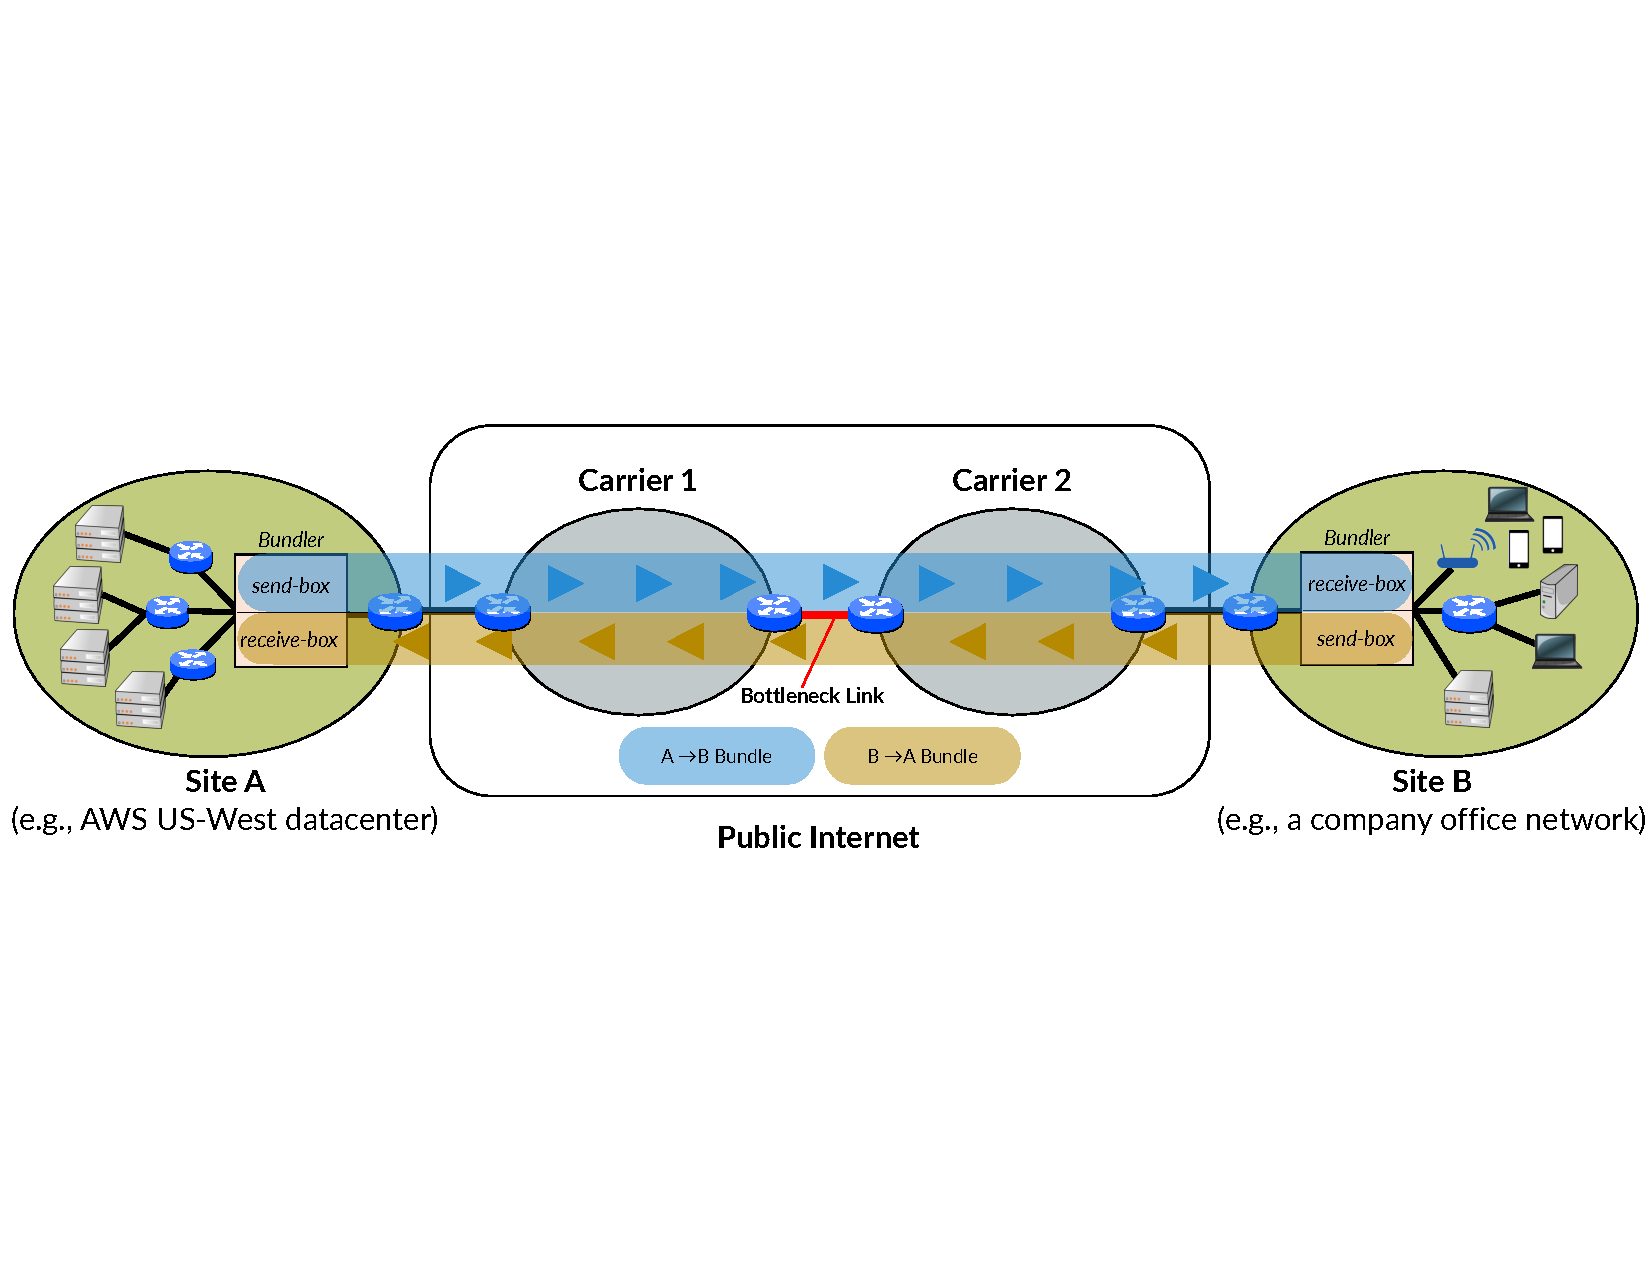
\includegraphics[width=\textwidth]{img/deployment-arch.pdf}
    \caption{An example deployment scenario for \name. 
    \name sits at each domain's edge. Traffic between the two boxes is aggregated into a single unidirectional bundle, shown as shaded boxes. The \inbox schedules the traffic within the bundle according to the policy the sending domain specifies (\S\ref{s:design}).
    \radhika{maybe remove the term `interdomain'? add a key for `A to B bundle' and `B to A bundle'.}}\label{fig:deploy:arch}
\end{figure*}

%We further note that middleboxes are now prevalent in the Internet architecture~\cite{aplomb}. They are often deployed at the egress and ingress of a network domain, to ensure traffic transits them for intrusion detection, packet inspection, filtering etc. They thus provide an effective vantage point for aggregating and managing traffic. 

We develop a new type of middlebox for this, called \name, that (1) aggregates the traffic leaving a sender's domain and destined to the same receiver's domain into appropriate bundles, (2) uses a delay-based congestion control algorithm to compute and enforce a sending rate for each bundle to move the corresponding queues from within the network to itself, and (3) applies scheduling and AQM policies within each bundle. 

%Our key insight (discussed in \S\ref{s:design}) is the bundle rate control mechanism: to move the queues, we can simply use a delay-controlling congestion control algorithm. \radhika{can i chop this?}
%\an{shouldn't we keep the key insight in the intro?}

As shown in Figure~\ref{fig:deploy:arch}, a \name middlebox implements sender-side and receiver-side functionality in a \emph{\inbox} and \emph{\outbox} respectively. The \inbox of one domain establishes a pairing with the \outbox of another domain when sending traffic to it. We thus define a \emph{bundle} to be a group of flows that share the same \inbox-\outbox pair.
The bulk of \name's functionality resides at the \inbox, which coordinates with the \outbox to identify bundles and measure congestion signals such as the round-trip time and the rate at which packets are received, and passes these signals to a delay-based congestion control algorithm (as described in \S\ref{s:design}) which computes appropriate sending rates.
%The \inbox passes these signals to a delay-based congestion control algorithm (as described in \S\ref{s:design}) which computes appropriate sending rates for each bundle, such that the queuing induced by the bundled traffic within the network is low and is incurred at the \inbox instead, while still maintaining high utilization at the bottleneck link.
We introduce a lightweight method for the coordination between the \inbox and the \outbox which does not require any per-flow state and can be deployed in a mode that forwards packets without modification.  \name requires no changes to the end hosts or to the routers in the network.
 
Note that our goal is to perform scheduling and queue management only on the traffic within the same bundle. We do not currently attempt to control traffic across different bundles. 
Furthermore, as we will discuss in \S\ref{s:deploy}, there may be instances where \name cannot improve performance for the bundled traffic, and falls back to the status quo performance; \ie the performance achieved today when queues build in the network instead of the edge. 
Despite these limitations, we believe that our work provides a deployable solution for enabling some of the benefits of scheduling and queue management in the Internet from the edge of the content provider's network.
 
We make the following contributions:
\begin{enumerate}
    \item A light-weight, scalable, and deployable architecture that enables content providers to perform scheduling across traffic with a common destination domain. In this architecture, content providers perform congestion control over bundles of traffic with a common destination domain in order to move queueing to the content provider's edge (\S\ref{s:design}).
     \item A novel low-overhead protocol-agnostic technique for measuring signals for congestion control between the \pair, that need not make any changes to the packet headers (\S\ref{s:measurement}).
     \item A new congestion controller, synthesized from existing building blocks in congestion control (delay-control~\cite{copa}, AQM~\cite{pie}, and cross-traffic inference\footnote{See Appendix \S\ref{s:app:nimbus}.}) for use with traffic bundles (\S\ref{s:queue-ctl}).
     %\item The design and implementation of a \name, including a novel method of collecting congestion control information and enforcing the decisions of a rate control algorithm on traffic aggregates, which \emph{moves} the queues from the bottleneck in the network to the customer's edge.
     %\item An evaluation of the benefits of scheduling and queue management for traffic aggregates, compared to both the status quo (FIFO) and an idealized deployment where bottleneck queues deploy the desired policy.
\end{enumerate}
